\documentclass{standalone}
\usepackage{tikz}
\usetikzlibrary{patterns}
\usetikzlibrary{positioning}
\usetikzlibrary{patterns, positioning}
\usetikzlibrary{shapes.misc}
\usepackage[outline]{contour}
\contourlength{1.5pt} 
\usepackage[sfdefault]{ClearSans}

\begin{document}
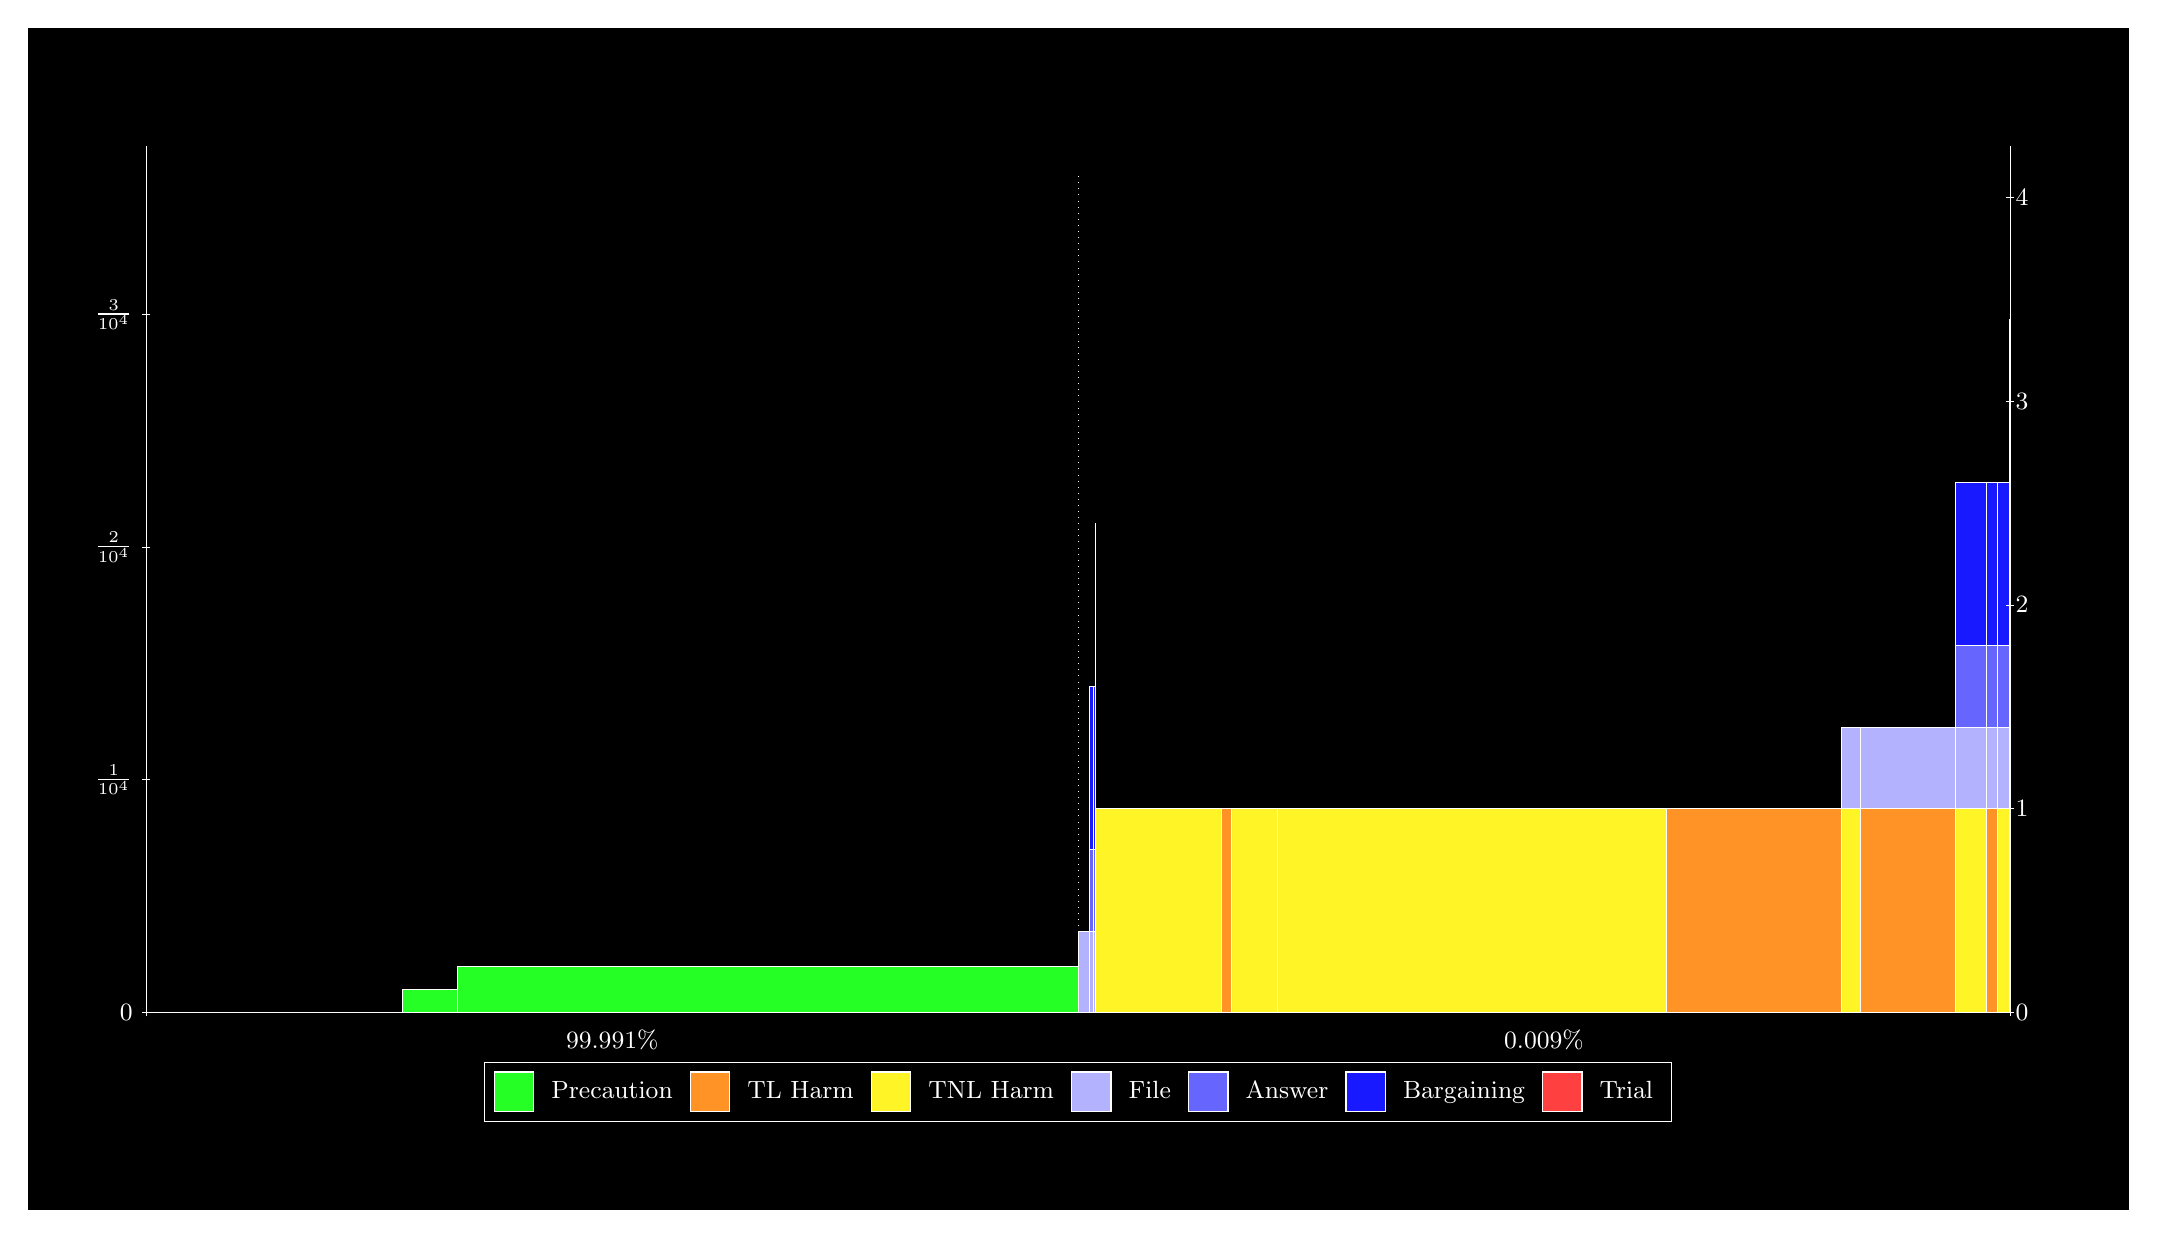
\begin{tikzpicture}
\draw[fill=black] (0,0) rectangle (26.667,15);
\draw[fill=green!85,draw=white,very thin] (4.7447,2.5) rectangle (5.4444,2.7955);
\draw[fill=green!85,draw=white,very thin] (5.4444,2.5) rectangle (13.333,3.0911);
\draw[fill=blue!30,draw=white,very thin] (13.333,2.5) rectangle (13.478,3.5353);
\draw[fill=blue!30,draw=white,very thin] (13.478,2.5) rectangle (13.531,3.5353);
\draw[fill=blue!60,draw=white,very thin] (13.478,3.5353) rectangle (13.531,4.5706);
\draw[fill=blue!90,draw=white,very thin] (13.478,4.5706) rectangle (13.531,6.6412);
\draw[fill=green!85,draw=white,very thin] (13.531,2.5) rectangle (13.547,2.5);
\draw[fill=blue!30,draw=white,very thin] (13.531,2.5) rectangle (13.547,3.5353);
\draw[fill=blue!60,draw=white,very thin] (13.531,3.5353) rectangle (13.547,4.5706);
\draw[fill=blue!90,draw=white,very thin] (13.531,4.5706) rectangle (13.547,6.6412);
\draw[fill=blue!30,draw=white,very thin] (13.547,2.5) rectangle (13.548,3.5353);
\draw[fill=blue!60,draw=white,very thin] (13.547,3.5353) rectangle (13.548,4.5706);
\draw[fill=blue!90,draw=white,very thin] (13.547,4.5706) rectangle (13.548,6.6412);
\draw[fill=red!75,draw=white,very thin] (13.547,6.6412) rectangle (13.548,8.7118);
\draw[fill=yellow!85,draw=white,very thin] (13.548,2.5) rectangle (15.149,5.0882);
\draw[fill=orange!85,draw=white,very thin] (15.149,2.5) rectangle (15.273,5.0882);
\draw[fill=green!85,draw=white,very thin] (15.273,2.5) rectangle (15.859,2.5);
\draw[fill=yellow!85,draw=white,very thin] (15.273,2.5) rectangle (15.859,5.0883);
\draw[fill=green!85,draw=white,very thin] (15.859,2.5) rectangle (20.805,2.5001);
\draw[fill=yellow!85,draw=white,very thin] (15.859,2.5001) rectangle (20.805,5.0883);
\draw[fill=green!85,draw=white,very thin] (20.805,2.5) rectangle (23.031,2.5001);
\draw[fill=orange!85,draw=white,very thin] (20.805,2.5001) rectangle (23.031,5.0883);
\draw[fill=yellow!85,draw=white,very thin] (23.031,2.5) rectangle (23.271,5.0882);
\draw[fill=blue!30,draw=white,very thin] (23.031,5.0882) rectangle (23.271,6.1235);
\draw[fill=orange!85,draw=white,very thin] (23.271,2.5) rectangle (24.477,5.0882);
\draw[fill=blue!30,draw=white,very thin] (23.271,5.0882) rectangle (24.477,6.1235);
\draw[fill=yellow!85,draw=white,very thin] (24.477,2.5) rectangle (24.869,5.0882);
\draw[fill=blue!30,draw=white,very thin] (24.477,5.0882) rectangle (24.869,6.1235);
\draw[fill=blue!60,draw=white,very thin] (24.477,6.1235) rectangle (24.869,7.1588);
\draw[fill=blue!90,draw=white,very thin] (24.477,7.1588) rectangle (24.869,9.2294);
\draw[fill=orange!85,draw=white,very thin] (24.869,2.5) rectangle (25.006,5.0882);
\draw[fill=blue!30,draw=white,very thin] (24.869,5.0882) rectangle (25.006,6.1235);
\draw[fill=blue!60,draw=white,very thin] (24.869,6.1235) rectangle (25.006,7.1588);
\draw[fill=blue!90,draw=white,very thin] (24.869,7.1588) rectangle (25.006,9.2294);
\draw[fill=green!85,draw=white,very thin] (25.006,2.5) rectangle (25.157,2.5);
\draw[fill=yellow!85,draw=white,very thin] (25.006,2.5) rectangle (25.157,5.0883);
\draw[fill=blue!30,draw=white,very thin] (25.006,5.0883) rectangle (25.157,6.1236);
\draw[fill=blue!60,draw=white,very thin] (25.006,6.1236) rectangle (25.157,7.1588);
\draw[fill=blue!90,draw=white,very thin] (25.006,7.1588) rectangle (25.157,9.2294);
\draw[fill=green!85,draw=white,very thin] (25.157,2.5) rectangle (25.16,2.5);
\draw[fill=orange!85,draw=white,very thin] (25.157,2.5) rectangle (25.16,5.0883);
\draw[fill=blue!30,draw=white,very thin] (25.157,5.0883) rectangle (25.16,6.1236);
\draw[fill=blue!60,draw=white,very thin] (25.157,6.1236) rectangle (25.16,7.1588);
\draw[fill=blue!90,draw=white,very thin] (25.157,7.1588) rectangle (25.16,9.2294);
\draw[fill=yellow!85,draw=white,very thin] (25.16,2.5) rectangle (25.163,5.0882);
\draw[fill=blue!30,draw=white,very thin] (25.16,5.0882) rectangle (25.163,6.1235);
\draw[fill=blue!60,draw=white,very thin] (25.16,6.1235) rectangle (25.163,7.1588);
\draw[fill=blue!90,draw=white,very thin] (25.16,7.1588) rectangle (25.163,9.2294);
\draw[fill=red!75,draw=white,very thin] (25.16,9.2294) rectangle (25.163,11.3);
\draw[fill=orange!85,draw=white,very thin] (25.163,2.5) rectangle (25.167,5.0882);
\draw[fill=blue!30,draw=white,very thin] (25.163,5.0882) rectangle (25.167,6.1235);
\draw[fill=blue!60,draw=white,very thin] (25.163,6.1235) rectangle (25.167,7.1588);
\draw[fill=blue!90,draw=white,very thin] (25.163,7.1588) rectangle (25.167,9.2294);
\draw[fill=red!75,draw=white,very thin] (25.163,9.2294) rectangle (25.167,11.3);
\draw[white,very thin] (1.5,2.5) -- (1.5,13.5);
\draw[white,very thin] (1.45,2.5) -- (1.55,2.5);
\node[font=\small,text=white, anchor=east] at (1.45, 2.5) {0};
\draw[white,very thin] (1.45,5.4554) -- (1.55,5.4554);
\node[font=\small,text=white, anchor=east] at (1.45, 5.4554) {$\frac{1}{10^{4}}$};
\draw[white,very thin] (1.45,8.4109) -- (1.55,8.4109);
\node[font=\small,text=white, anchor=east] at (1.45, 8.4109) {$\frac{2}{10^{4}}$};
\draw[white,very thin] (1.45,11.366) -- (1.55,11.366);
\node[font=\small,text=white, anchor=east] at (1.45, 11.366) {$\frac{3}{10^{4}}$};

\draw[white,dotted,very thin] (13.333,2.83) -- (13.333,13.17);
\draw[white,very thin] (25.167,2.5) -- (25.167,13.5);
\draw[white,very thin] (25.117,2.5) -- (25.217,2.5);
\node[font=\small,text=white, anchor=west] at (25.117, 2.5) {0};
\draw[white,very thin] (25.117,5.0882) -- (25.217,5.0882);
\node[font=\small,text=white, anchor=west] at (25.117, 5.0882) {1};
\draw[white,very thin] (25.117,7.6765) -- (25.217,7.6765);
\node[font=\small,text=white, anchor=west] at (25.117, 7.6765) {2};
\draw[white,very thin] (25.117,10.265) -- (25.217,10.265);
\node[font=\small,text=white, anchor=west] at (25.117, 10.265) {3};
\draw[white,very thin] (25.117,12.853) -- (25.217,12.853);
\node[font=\small,text=white, anchor=west] at (25.117, 12.853) {4};

\draw[white,very thin] (1.5,2.5) -- (25.167,2.5);
\draw[white,very thin] (1.5,2.45) -- (1.5,2.55);
\node[font=\small,text=white, anchor=north] at (1.5, 2.45) {};
\draw[white,very thin] (25.167,2.45) -- (25.167,2.55);
\node[font=\small,text=white, anchor=north] at (25.167, 2.45) {};

\node[font=\small,text=white,anchor=south] at (7.4167, 1.9) {99.991\%};
\node[font=\small,text=white,anchor=south] at (19.25, 1.9) {0.009\%};
\draw (13.3333,2.5) node (B) {};
\begin{scope}[align=center]
\matrix[scale=0.5,draw=white,below=0.5cm of B,nodes={draw},column sep=0.1cm]{
\node[rectangle,draw,minimum width=0.5cm,minimum height=0.5cm,fill=green!85]{}; & \node[draw=none,font=\small,text=white]{Precaution}; &
\node[rectangle,draw,minimum width=0.5cm,minimum height=0.5cm,fill=orange!85]{}; & \node[draw=none,font=\small,text=white]{TL Harm}; &
\node[rectangle,draw,minimum width=0.5cm,minimum height=0.5cm,fill=yellow!85]{}; & \node[draw=none,font=\small,text=white]{TNL Harm}; &
\node[rectangle,draw,minimum width=0.5cm,minimum height=0.5cm,fill=blue!30]{}; & \node[draw=none,font=\small,text=white]{File}; &
\node[rectangle,draw,minimum width=0.5cm,minimum height=0.5cm,fill=blue!60]{}; & \node[draw=none,font=\small,text=white]{Answer}; &
\node[rectangle,draw,minimum width=0.5cm,minimum height=0.5cm,fill=blue!90]{}; & \node[draw=none,font=\small,text=white]{Bargaining}; &
\node[rectangle,draw,minimum width=0.5cm,minimum height=0.5cm,fill=red!75]{}; & \node[draw=none,font=\small,text=white]{Trial}; \\\\
};\end{scope}

\end{tikzpicture}
\end{document}